    \documentclass[11pt]{article}
    \usepackage[pdftex]{graphicx}
    \usepackage{times}
    \fontsize{9}{11}
    \usepackage{cite}
    \usepackage{lineno}
    \usepackage{amsmath,amssymb,amsthm}
    \usepackage{rotating}
    \usepackage[usenames]{color}
    \newcommand{\captionfonts}{\small}
    \usepackage{authblk}
    \usepackage[left=1in,top=1in,right=1in,bottom=1in]{geometry}
    \linespread{1.5}

    \usepackage[footnotesize]{caption}
    \renewcommand\Affilfont{\small}
     
\begin{document}

\textbf{Electronic Supplementary Material for ``Evolutionary Decomposition and the Mechanisms of Cultural Change"}\\
Bret A. Beheim, Ryan Baldini\\

Table of Contents\\
I. Extended Analysis of Individual Change Term\\
II. Analysis of RS Term\\
III. Analysis of Death Term\\
IV. SnoobSim Documentation\\

All models below were coded in R using variables extracted from the 54 SnoobSim census records.  Models were fit by maximum likelihood using the function \texttt{mle2} in Ben Bolker's \texttt{bbmle} package (cran.r-project.org/), with the default BFGS algorithm.\\

\textbf{I. Extended Analysis of Individual Change}\\

The ``individual change'' decomposition bars indicate that initially the balance of change is negative and large in magnitude.  As the frequency of Snoobs approaches 50\%, though, this effect becomes smaller and smaller, and as Snoobs move towards fixation the effect reverses and the balance of converts is now strongly positive, at times rivaling RS in magnitude.

An important thing to keep in mind when reading the individual change bars is that they represent only the average phenotypic cange across individuals; some individuals became Snoobs in the first few decades, but more apostatised to non-Snoob.  

Our outcome variable here is ``will be a Snoob'' in the next census ($\phi_{i,t+1}$), modeled by current Snoob status and other properties of individuals and the population.  Because we have a binary outcome variable, we use a binomial model with various parameterizations of $p$.  A standard way to express this probability is the form $p = LM + (1-L)\phi_{i,t}$, so individuals update with probability $L$ and retain their current status with probability $(1-L)$.  Strictly speaking, this sequence of first updating, then (potentially) changing phenotype implied by this model is quite artificial for real human learning.  However, it is interesting to consider human cultural change \textit{as if} it proceeded in this fashion, because the updating rule can incorporate a variety of hypothesized mechanisms for comparison using information criteria. 

The simplest model is a constant Snoob conversion probability for all individuals
	\[M_0 = \alpha.
\]
In other words, individuals update with probability $L$, and of those we expect fraction $\alpha$ take Snoobism as their phenotype.

Conformist learning is parameterized in four, very similar, ways.  The model $\overline{\phi}_t + D(2\overline{\phi}_t-1) \overline{\phi}_t (1-\overline{\phi}_t)$ is Boyd and Richerson's \cite{boyd1985culture} model.  Parameter $D$ represents the strength of conformity; $D=0$ indicates no conformity and unbiased, frequency-dependent learning.  If $D > 0$, conformity will increasingly dominate the probability of becoming a Snoob, while $D < 0$ implies non-conformity (you are more likely to choose the opposite of the majority's trait).  Bowles \cite{bowles2006microeconomics} modifies this by creating an explicit parameter for the threshold, allowing it to vary from 0.5, so which we could write as $\overline{\phi}_t + D(2\overline{\phi}_t-2k)\overline{\phi}_t(1-\overline{\phi}_t)$.  The conformity model in McElreath, et al. \cite{mcelreath2008beyond}\footnote{The basic form of this model was suggested to McElreath et al. by Sam Bowles (Richard McElreath, \textit{personal communication}).} expresses a similar idea, using the model
	\[ M_1 = \frac{\overline{\phi}_t^\beta}{\overline{\phi}_t^\beta + (1-\overline{\phi}_t)^\beta}
\]
where $\beta > 1$ represents conformity.  Because the Boyd and Richerson model is actually Taylor series approximation of this more general model when $\beta$ is close to 1 and $\overline{\phi}_t$ is near 0.5, we may sensibly write all three models in a common notation.  Hence, in our analysis, we include the 1985 model as
	\[ M_2 = \overline{\phi}_t + 2(\beta-1)(2\overline{\phi}_t-1),
\]
and the 2004 model as
	\[ M_3 = \overline{\phi}_t + 2(\beta-1)(2\overline{\phi}_t-2k).
\]
Another sensible way to parameterize conformity is by using a logit link function, such that
	\[ M_4 = \mathrm{logit}^{-1}(\alpha + \beta \overline{\phi}_t) = \frac{\exp(\alpha + \beta \overline{\phi}_t)}{1 + \exp(\alpha + \beta \overline{\phi}_t)}. \]

Two density-dependent models, one with a quadratic effect,
	\[ M_5 = \mathrm{logit}^{-1}(\alpha + \beta N_t),\]
	\[ M_6 = \mathrm{logit}^{-1}(\alpha + \beta_1 N_t + \beta_2 N_t^2).\]
Model $M_6$ used population sizes coded in standard units, to aid the maximum likelihood algorithm. Two time series models, one with a quadratic effect,
	\[ M_7 = \mathrm{logit}^{-1}(\alpha + \beta t),\]
	\[ M_8 = \mathrm{logit}^{-1}(\alpha + \beta_1 t + \beta_2 t^2 ).\]
Oscillatory models of time and population were also used:
	\[ M_9 = \mathrm{logit}^{-1}(\alpha + \beta_1 \sin (\beta_2 t)),\]
	\[ M_{10} = \mathrm{logit}^{-1}(\alpha + \beta_1 \sin (\beta_2 N_t)).\]
Various combinations were also included.  Including time and population size,
\[ M_{11} = \mathrm{logit}^{-1}(\alpha + \beta_1 t + \beta_2 N_t).\]
Including population Snoob frequency, individual age in years (centered on mean), and gender (coded as a 1/0 variable ``male''),
\[ M_{12} = \mathrm{logit}^{-1}(\alpha + \beta_1 \overline{\phi}_t + \beta_2 \mathrm{male} + \beta_3 \mathrm{age}).\]
The final model included adds time to model $M_{12}$,
\[ M_{13} = \mathrm{logit}^{-1}(\alpha + \beta_1 \overline{\phi}_t + \beta_2 \mathrm{male} + \beta_3 \mathrm{age} + \beta_4 t).\]

Running a model comparison ranks these thirteen models according to Table \ref{tab:ichangemodels}.  Schwartz criterion ranks (BIC) are nearly identical to AIC$_c$ ranks, nominating models $M_1$ and $M_2$ as the best-performing.  The constant model, $M_0$, performs worst among the model set, but conformity models completely dominate the model weighting.  This would indicate that the best out-of-sample predictive models as identified by information theory are purely social learning models using $\overline{\phi}_t$, and do not improve by adding other population-level covariates like population size, or individual-level variables like gender or age.

 
\begin{table}[htbp]
  \centering
    \begin{tabular}{lrrrrr}
  	\hline
  	\hline
    Model & $k$ & AIC$_c$ weight & BIC weight & $\Delta$ AIC$_c$ & $\Delta$ BIC \\
   	\hline
    $M_2$  & 2     & 40.49\% & 50.10\% & 0.00  & 0.00 \\
    $M_1$  & 2     & 40.19\% & 49.72\% & 0.02  & 0.02 \\
    $M_3$  & 3     & 17.44\% & 0.17\% & 1.69  & 11.42 \\
    $M_4$  & 3     & 1.06\% & 0.01\% & 7.28  & 17.02 \\
    $M_{12}$ & 5     & 0.58\% & 0.00\% & 8.48  & 37.68 \\
    $M_{13}$ & 6     & 0.24\% & 0.00\% & 10.27 & 49.21 \\
    $M_6$  & 4     & 0.00\% & 0.00\% & 67.35 & 86.82 \\
    $M_8$  & 4     & 0.00\% & 0.00\% & 102.91 & 122.38 \\
    $M_7$  & 3     & 0.00\% & 0.00\% & 107.40 & 117.14 \\
    $M_5$  & 3     & 0.00\% & 0.00\% & 921.84 & 931.57 \\
    $M_{11}$ & 4     & 0.00\% & 0.00\% & 1070.58 & 1090.05 \\
    $M_{10}$ & 4     & 0.00\% & 0.00\% & 2007.97 & 2027.44 \\
    $M_9$  & 4     & 0.00\% & 0.00\% & 2254.17 & 2273.64 \\
    $M_0$  & 1     & 0.00\% & 0.00\% & 133107.95 & 133098.21 \\
    \hline
    \end{tabular}%
    \caption{Individual change updating models, by AIC$_c$ rank, with AIC$_c$ and BIC scores in terms of the top model, $M_2$, and model weights (all to two decimal places).  Both the Akaike Information Criterion and the Schwartz Criterion (BIC) rank the performance of each model by assigning penalties to its MLE likelihood value; AIC and AIC$_c$ penalize by the number of parameters, $k$, in a given model.}
  \label{tab:ichangemodels}%
\end{table}%

Because of the functional similarity between $M_1$, $M_2$, and $M_3$, the parameter estimates are nearly identical, and only $M_1$ will be discussed.  The conformity coefficient (with standard error) was estimated as 1.374 (0.028), which, being above 1, is evidence towards conformist biased updating.  The maximum-likelihood estimate for the intercensus updating probability, $L$, was 0.100 (0.002), meaning that under this model about 10\% of the population updates every five years, while 90\% do not update at all.  It is worth noting these estimates are quite sensible per what the SnoobSim software is actually doing (next section).

\begin{figure}[t]
\begin{center}
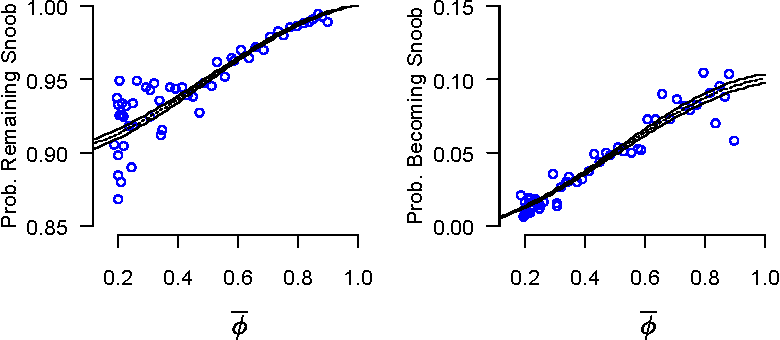
\includegraphics[scale=1]{ichange.pdf}
\caption{Fitted model $M_1$ plotted over the observed proportions of individuals who will switch to or remain Snoobs intercensus, on the population Snoob frequency for the first 53 censuses.  Maximum likelihood estimates (dashed line) and 95\% HPDI intervals (solid lines) for the Bernoulli probability of becoming a Snoob, $p$, show a strong nonlinear association between individual change and $\overline{\phi}_t$.}
\label{fig:ichange}
\end{center}
\end{figure}





\newpage
\textbf{Individual Change - What SnoobSim is Actually Doing}\\

In the simulation, each day, some fraction of the population decides they will ``update'' their Snoob status.  To be precise, each individual updates daily with probability 0.00006.  If an individual decides to update, they then collect a random sample of 100 people in the population, and uses this information to decide to change their Snoob status or stay where they are.  Note that once an individual decides to update, their previous Snoob status becomes irrelevant.  Each individual takes their particular sample of 100 and adopts Snoobism with probability given by the code:

\begin{verbatim}
prob.converting.to.snoob <- 
	(sample.frq^conformity.bias.snoob)/
	(sample.frq^conformity.bias.snoob	+ (1-sample.frq)^conformity.bias.snoob)
\end{verbatim}

In other words, learners used exactly the same mechanism as $M_1$, except on the Snoob frequency among the 100 they randomly sampled, rather than the population frequency.  No surprise, then, that models with this functional form came in first in the model comparison.  The simulation parameter \texttt{conformity.bias.snoob} was set to 1.3 (compare against the MLE of $\beta$ above), and with a daily probability of updating set to 0.00006, we expect proportion $1-(1-0.00006)^{365\times5}=0.104$ of the population to update (compare to the MLE of $L$, above).  We should not expect real census data to nominate such simple models, but the utility of information-theoretic model comparison remains the same nonetheless.


\newpage
\textbf{I. Analysis of RS Term}\\

The strong, consistently positive effect of RS in the decomposition indicates that Snoobs have more children than non-Snoobs, on the average.  This could be causal, meaning Snoobism itself may have some effect on one's desire or ability to mate, or it could be a consequence of Snoobism covarying with some other trait.  For example, if people tend to become Snoobs during their reproductive careers, only to abandon it later in life, we would see a consistent, positive effect in the decomposition.  Or, perhaps Snoobism is a sex-specific trait and there are fewer of that gender in the population (so they must have higher mean RS).  

Hence, it is premature to say Snoobism is ``under selection'' without conclusive evidence against confounding variables.  This is difficult to impossible in observational contexts, like this one, but statistical control can at least tell us if the RS advantage of Snoobs remains when comparing Snoobs and non-Snoobs of the same gender and age.  

Our outcome variable is the number of kids an individual sires (if they are of reproductive age) have during the next intercensus period, which in our data varies between 0 and 8 (women are constrained to about 5 or 6 children in a five-year intercensus period), $f_{i, t+1}$.  We have some flexibility with count data, so we have chosen to compare models of the outcome variable using three possible probability distributions: geometric, Poisson, and zero-inflated Poisson.  For the Poisson family, $\lambda$ is modeled by an exponential link function ($\lambda = \exp(M)$, for some model $M$), while for the geometric models, the Bernoulli probability of success $p$ is modeled generically by logit link function ($p=\mathrm{logit}^{-1}(M)$).  

Altogether, twelve models of the expected number of intercensus children were compared.  Note that all uses of age center the variable on its mean.

	\[M_0 = \beta_0
\]
	\[M_1 = \beta_0 + \beta_1 \mathrm{age}
\]
	\[M_2 = \beta_0 + \beta_1 \mathrm{age} + \beta_2 \mathrm{(age)}^2
\]
	\[M_3 = \beta_0 + \beta_1 \mathrm{age} + \beta_2 \mathrm{(age)}^2 + \beta_3 \phi_{i,t}
\]
	\[M_4 = \beta_0 + \beta_1 \mathrm{age} + \beta_2 \mathrm{(age)}^2 + \beta_3 \phi_{i,t} + \beta_4 \mathrm{male}
\]
	\[M_5 = (1-N_t/K)(\beta_0 + \beta_1 \mathrm{age} + \beta_2 \mathrm{(age)}^2 + \beta_3 \phi_{i,t} + \beta_4 \mathrm{male})
\]
	\[M_6 = \exp(-K*N_t)(\beta_0 + \beta_1 \mathrm{age} + \beta_2 \mathrm{(age)}^2 + \beta_3 \phi_{i,t} + \beta_4 \mathrm{male})
\]
	\[M_7 = \beta_0 + \beta_1 \mathrm{age} + \beta_2 \overline{\phi}_t
\]
	\[M_8 = \beta_0 + \beta_1 \mathrm{age} + \beta_2 \mathrm{(age)}^2 + \beta_3 \overline{\phi}_t
\]
	\[M_9 = \beta_0 + \beta_1 \mathrm{age} + \beta_2 \mathrm{(age)}^2 + \beta_3 \phi_{i,t} + \beta_4 \overline{\phi}_t
\]
	\[M_{10} = \beta_0 + \beta_1 \mathrm{age} + \beta_2 \mathrm{(age)}^2 + \beta_3 \phi_{i,t} + \beta_4 \mathrm{male} + \beta_5 \overline{\phi}_t
\]
	\[M_{11} = \beta_0 + \beta_1 \mathrm{age} + \beta_2 \mathrm{(age)}^2 + \beta_3 \phi_{i,t} + \beta_4 \mathrm{male} + \beta_5 (\mathrm{male} \times \phi_{i,t})
\]
	\[M_{12} = \beta_0 + \beta_1 \mathrm{age} + \beta_2 \mathrm{(age)}^2 + \beta_3 \phi_{i,t} + \beta_4 \mathrm{male} + \beta_5 \overline{\phi}_t + \beta_6 (\mathrm{male} \times \phi_{i,t})
\]

Since each of these 12 models can be placed within a Poisson, geometric, or zero-inflated Poisson (ZIP) distribution, a total of 36 distinct models are fitted separately to the data and compared for out-of-sample predictive accuracy using AIC$_c$ and BIC (Table \ref{tab:RScompare}).

The top models, $M_{10}$ and $M_{12}$, both include age, gender and Snoob status, and differ only in an interaction effect between male and Snoob status.  No density-dependent or frequency-dependent models performed as well.  Also, according to the model comparison, the zero-inflated Poisson distribution is the best-performing stochastic wrapper around these two models, as opposed to the geometric distribution or the Poisson, which are vastly outperformed.

Estimates and confidence intervals for $M_{10}$ are presented in table \ref{tab:m10ests}, with MLE-fitted lines plotted in Figure \ref{fig:rs}.  It is clear from the estimates and figure that Snoobism remains an excellent predictor of reproductive output after accounting for age and gender.  This allows us to rule out the possibility that the decomposition results for RS were merely a consequence of chance associations between Snoobism and age or gender, and points to the possibility Snoobism is under some form of fecundity or sexual selection.    

\begin{table}[htbp]
  \centering
    \begin{tabular}{lcrrrr}
    \hline
    \hline
    Parameter & Estimate & Std. Error & 2.50\% & 97.50\% \\
    \hline
    $\beta_0$    & -0.878 & 0.024 & -0.924 & -0.831 \\
    $\beta_1$    & -0.006 & 0.000 & -0.007 & -0.005 \\
    $\beta_2$    & -0.002 & 0.000 & -0.003 & -0.002 \\
    $\beta_3$    & 0.681 & 0.017 & 0.647 & 0.714 \\
    $\beta_4$    & 0.120 & 0.013 & 0.093 & 0.147 \\
    $\beta_5$    & 0.244 & 0.033 & 0.179 & 0.309 \\
    $\alpha$ & 0.357 & 0.006 & 0.3451 & 0.369 \\
    \hline
    \end{tabular}%
    \caption{Parameter estimates for the zero-inflated Poisson version of model $M_{10}$.  The second-placed model's fitted values are nearly identical to these but with an additional interaction term for Male snoobs of -0.043 (0.030), MLE and SE.  Parameter $\alpha$ estimates the frequency an outcome of 0 will be drawn from the distribution, beyond what would be expected by the Poisson model.} 
  \label{tab:m10ests}%
\end{table}%

\begin{table}[htbp]
  \centering
    \begin{tabular}{llrrrrr}
    \hline
    \hline
    Model & Distribution & $k$ & AIC$_c$ weight & BIC weight & $\Delta$ AIC$_c$ & $\Delta$ BIC \\
    \hline
    $M_{10}$ & ZIP   & 7     & 72.35\% & 99.63\% & 0.00  & 0.00 \\
    $M_{12}$ & ZIP   & 8     & 27.65\% & 0.37\% & 1.92  & 11.17 \\
    $M_{12}$ & Geom. & 7     & 0.00\% & 0.00\% & 28.19 & 28.19 \\
    $M_{10}$ & Geom. & 6     & 0.00\% & 0.00\% & 36.98 & 27.73 \\
    $M_4$  & ZIP   & 6     & 0.00\% & 0.00\% & 52.23 & 42.98 \\
    $M_{11}$ & ZIP   & 7     & 0.00\% & 0.00\% & 53.70 & 53.70 \\
    $M_{11}$ & Geom. & 6     & 0.00\% & 0.00\% & 72.55 & 63.30 \\
    $M_{4}$ & Geom. & 5     & 0.00\% & 0.00\% & 80.50 & 62.00 \\
    $M_3$  & Geom. & 4     & 0.00\% & 0.00\% & 98.63 & 70.87 \\
    $M_3$  & ZIP   & 5     & 0.00\% & 0.00\% & 129.07 & 110.57 \\
    $M_8$  & Geom. & 4     & 0.00\% & 0.00\% & 1553.27 & 1525.52 \\
    $M_8$  & ZIP   & 5     & 0.00\% & 0.00\% & 1699.65 & 1681.15 \\
    $M_{12}$ & Poisson & 7     & 0.00\% & 0.00\% & 1779.76 & 1779.76 \\
    $M_{10}$ & Poisson & 6     & 0.00\% & 0.00\% & 1795.46 & 1786.21 \\
    \hline
    \end{tabular}%
    \caption{Models of reproductive success, by AIC$_c$ and BIC rankings to two decimal places.  Models can appear more than once in the rankings because they are embedded in different stochastic nodes: the second-ranked model is $M_{12}$ in a zero-inflated Poisson distribution (ZIP), while the third-ranked model is $M_{12}$ in a geometric distribution.  Of the 36 models tested (three stochastic distributions for each of twelve structural models), only the top 14 are shown.}
  \label{tab:RScompare}%
\end{table}%


\begin{figure}[t]
\begin{center}
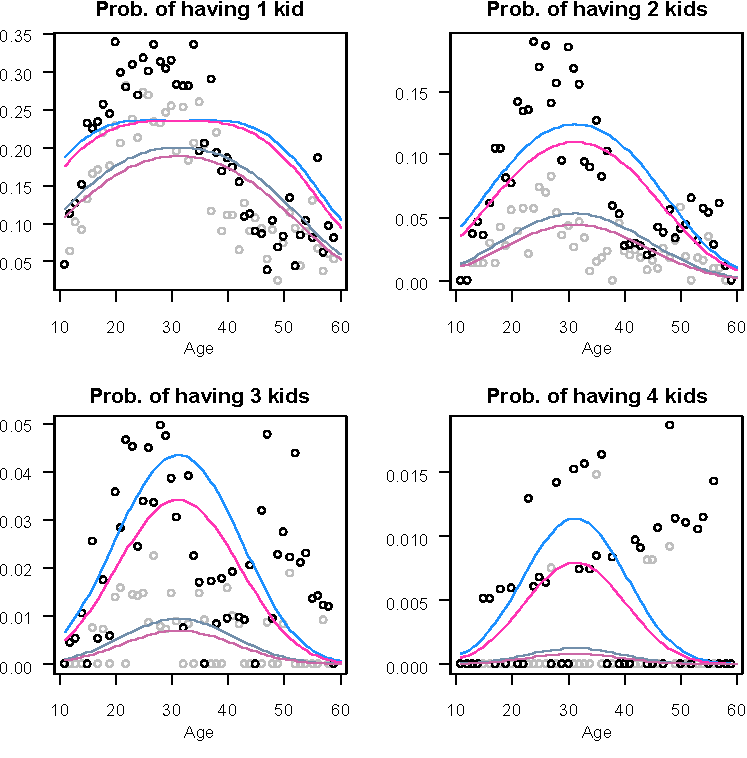
\includegraphics[scale=1]{rs.pdf}
\caption{Fitted model $M_{10}$ plotted over the observed proportions of parents with exactly a certain number of intercensus children, by parent age.  For each of the 53 intercensus periods, Snoobs (black circles) have more children on average than non-Snoobs (gray circles), which reflected by the fitted lines as well.  Snoob men (bright blue) have more children on average than both Snoob women (bright pink) and non-Snoob men (dark blue), implying a sex-ratio imbalance.}
\label{fig:rs}
\end{center}
\end{figure}




\newpage
\textbf{Reproductive Success: What SnoobSim is Actually Doing}\\

Women become pregnant probabilistically according to an age-specific fertility schedule identical to that of a realistic population (US women c. 2005).  From the ages of 15 to 50, women reference a daily probability of conception given by

\begin{verbatim}
daily.pr.conception <- (1-(1/(1+exp(alpha + beta1*snoob))))
\end{verbatim}

Parameter \texttt{alpha} is set by the fertility schedule, and the effect of being a Snoob is for this run is \texttt{beta1}=0.8, exaggerating a Snoob's age-specific fertility schedule and increasing the daily probability she will become pregnant.  If a woman conceives, she will then choose a male as the father.  

Men are promiscuous and can be chosen by multiple women (one lucky man fathered a record 8 kids in 5 years with several different women).  Women will continue to mate with the same man until he becomes unavailable due to advanced age (i.e. greater than 60 years old) or death.

According to the simulator parameters, women almost always choose males who are like them with respect to Snoob status.  Men enjoy no specific fertility schedule, but because of this positive assortment we can expect Snoob men will have different fertility schedules than nonSnoob men.  However, a man's age (or any other traits for that matter) has nothing to do with his being selected, so we should not expect a male's age-specific fertility to be like a female's.  Nevertheless, mechanistically Snoobism has a direct impact on one's RS, and this effect cannot be controlled out by including other covariates.  As far as the simulation is concerned, Snoobism is indeed under strong fertility selection.


\newpage
\textbf{III. Analysis of Mortality Term}\\

According to the RTDICE decomposition, non-Snoobs die more than Snoobs, causing Snoobism to consistently increase by a relatively small amount.  As with positive RS, this could be a result of a behavior consequent from Snoobism itself, in which case we could say the positive mortality effect is ``viability selection''.  But, alternatively, this effect could be due to an association between Snoobism and some other trait which confers differential survival.  For example, if young people are more attracted to Snoobism, while seniors tend to dismiss it as a folly of youth, Snoobism would negatively covary with mortality despite having no mechanistic effect on one's mortality.
                            
Our goal, then, is to establish whether Snoob status still helps predict mortality outcomes even after accounting for age, gender, and other relevant life history characteristics.  This motivates a number of mortality models.  Because we can work with individual-level data for multiple time periods, we specifically wish to model whether in the next intercensus period an individual will die ($d_{i,t+1} = 1$) or not ($d_{i,t+1}=0$), using their gender, age, and Snoob status, and possibly properties of the population.  This outcome is modeled as a binomial random variable, or $d_{i,t+1} \sim \mathrm{Binomial}(1,p)$, with $p$ taking the form of an inverse logit link of some model $M$.

A total of six models were included in this analysis:
	\[M_0 = \alpha
\]
	\[M_1 = \alpha + \beta_1 \mathrm{age}
\]
	\[M_2 = \alpha + \beta_1 \mathrm{age} + \beta_2 \mathrm{(age)}^2
\]
	\[M_3 = \alpha + \beta_1 \mathrm{age} + \beta_2 \mathrm{(age)}^2 + \beta_3 \mathrm{male}
\]
	\[M_4 = \alpha + \beta_1 \mathrm{age} + \beta_2 \mathrm{(age)}^2 + \beta_3 \mathrm{male} + \beta_4 \phi_{i,t}
\]
	\[M_5 = \alpha + \beta_1 \mathrm{age} + \beta_2 \mathrm{(age)}^2 + \beta_3 \mathrm{male} + \beta_4 \phi_{i,t} + \beta_5 \overline{\phi}_t
\]

Because long-lived humans record many zeros for this variable until their eventual death, we also considered a zero-inflated binomial stochastic node with the same logit-linked models of $p$, for a total of 12 models.  Comparing these as before produces Table \ref{tab:morttab}, which shows one clear winner: $M_4$ for the binomial distribution.  In other words, the information criteria suggest that the best way to predict one's mortality status is by knowing their age, gender, Snoob status together.  Plotting this fitted model on proportions of individuals who die at particular ages produces Figure \ref{fig:mortality}.  The $M_4$ are not perfect, but correctly identify the different mortality experiences across the lifetime for Snoob and non-Snoob.  As with RS, we can show clearly that Snoobism remains a useful predictor even accounting for age and gender, which may indicate that viability selection is in play in the mortality term in the decomposition.  



\begin{figure}[t]
\begin{center}
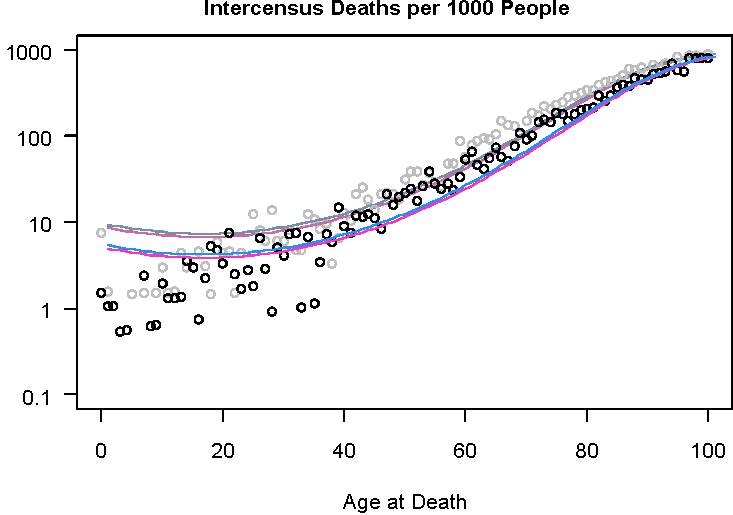
\includegraphics[scale=1]{mortality.pdf}
\caption{Fitted model $M_{4}$ plotted over the observed proportion of intercensus deaths per 1000 people by age.  For each of the 53 intercensus periods, Snoobs (black circles) die less frequently than non-Snoobs (gray circles), which reflected by the fitted lines as well.  Snoob women (bright pink) survive most frequently, closely followed by Snoob men (bright blue).  Non-Snoob men (dark blue) die most frequently of all, but at rates comparable to non-Snoob women (dark pink).}
\label{fig:mortality}
\end{center}
\end{figure}


% Table generated by Excel2LaTeX from sheet 'mort'
\begin{table}[htbp]
  \centering
  
    \begin{tabular}{llrrrrr}
    \hline
    \hline
    Model & Distribution & $k$     & AIC$_c$ weight & BIC weight & $\Delta$ AIC$_c$ & $\Delta$ BIC \\
    \hline
    $M_4$    & binomial & 5     & 100.00\% & 99.99\% & 0.00  & 0.00 \\
    $M_5$   & ZIB   & 7     & 0.00\% & 0.00\% & 20.41 & 39.87 \\
    $M_5$    & binomial & 6     & 0.00\% & 0.00\% & 21.20 & 30.94 \\
    $M_1$    & binomial & 2     & 0.00\% & 0.01\% & 47.62 & 18.41 \\
    $M_3$    & binomial & 4     & 0.00\% & 0.00\% & 49.82 & 40.08 \\
    $M_4$   & ZIB   & 6     & 0.00\% & 0.00\% & 76.98 & 86.71 \\
    $M_2$    & binomial & 3     & 0.00\% & 0.00\% & 122.52 & 103.05 \\
    $M_2$   & ZIB   & 4     & 0.00\% & 0.00\% & 309.24 & 299.50 \\
    $M_3$   & ZIB   & 5     & 0.00\% & 0.00\% & 717.33 & 717.33 \\
    $M_1$   & ZIB   & 3     & 0.00\% & 0.00\% & 1349.15 & 1329.68 \\
    $M_0$    & binomial & 1     & 0.00\% & 0.00\% & 15489.56 & 15450.62 \\
    $M_0$   & ZIB   & 2     & 0.00\% & 0.00\% & 15491.56 & 15462.36 \\
    \hline
    \end{tabular}%
    \caption{Model rankings for mortality models, with number of parameters ($k$).  To two decimal places, model $M_4$ completely dominates the information criterion weightings.}
  \label{tab:morttab}%
\end{table}%


\begin{table}[htbp]
  \centering
    \begin{tabular}{lcrrrr}
    \hline
    \hline
    Parameter & Estimate & Std. Error & 2.50\% & 97.50\% \\
    \hline
    $\alpha$    & 4.673 & 0.040 & 4.595 & 4.750 \\
    $\beta_1$    & -0.036 & 0.001 & -0.039 & -0.034 \\
    $\beta_2$    & -0.001 & 0.000 & -0.001 & -0.001 \\
    $\beta_3$    & -0.088 & 0.034 & -0.155 & -0.021 \\
    $\beta_4$    & 0.559 & 0.034 & 0.492 & 0.627 \\
    \hline
    \end{tabular}%
    \caption{Parameter estimates for model $M_{4}$ in a binomial model of mortality.  Snoob status substantially reduces the probability one will die at any given age or gender.} 
  \label{tab:m10ests}%
\end{table}%




\textbf{Mortality - What SnoobSim is Actually Doing}\\

Snoobs reference a different mortality schedule in the simulation specific to their age and gender.  The baseline mortality schedule for non-Snoobs is the estimated US mortality schedule c. 2005.  To be specific, the daily probability of death for each individual is calculated via:

\begin{verbatim}
daily.pr.death <- (1-(1/(1+exp(alpha + mortality.bias.male*male 
                                       + mortality.bias.snoob*snoob))))
\end{verbatim}

The parameter alpha represents the mortality schedule, but can be modified by both gender and Snoob status.  For this simulation, \texttt{mortality.bias.snoob} was set to -0.5, meaning Snoobs die less often, and and the \texttt{mortality.bias.male} was 0.3, meaning males die more often.  As a consequence, Snoobs should always die less for any given age and gender, and so the effects of this ``viability selection'' should show up in models that account for Snoob status.  





\newpage
\textbf{IV. SnoobSim Documentation}\\

SnoobSim is an agent-based population simulator in R that can be used to simulate virtually any demographic process in small populations.  It works by running through a daily list of stochastic events within the population and updating a master population register based on the outcome of these events, which can be influenced by the user.  Because population changes over decades, centuries, or longer can be simulated, a full record of every event inside the simulation is not intended to be saved.  Rather, the simulator records and exports census records taken in intervals specified by the researcher (e.g. every five years).  When it is time for another census, a copy of the population register for that day is saved, and when the simulation ends all such censuses are saved in csv format, as real field data would be stored.
  
Control of the simulator is managed through the ``control panel", a list of parameters at the top of the SnoobSim.r script.  These are divided into basic simulator values, such as the time between each census, initial population size, etc, vital population rates, such as age-specific fertility and mortality, etc. and evolutionary mechanisms, which control how the phenotypic traits of each individual are determined, and how they influence demographic parameters.  

Each day, the following demographic processes occur in this order:\\
1.	immigration \\
2.	births\\
3.	matings\\
4.	deaths\\
5.	emigration\\
6.	social learning / individual change\\

Since the simulation loops over days, which have relatively few births and deaths for realistic human populations, we expect that there are no important difficulties introduced by this order, or important differences if the order were changed.  

Immigration is controlled by two functions - \texttt{daily.immigration} and \texttt{immigrant.maker}.  The first determines how many individuals will immigrate into the population that day, following the crude immigration rate specified by the user.  If there are indeed immigrants that day, the \texttt{immigrant.maker} function will create new entries in the population register for each of them. 

Mating occur only if there are fecund males and females.  Any female between 15 and 50 years old who is not currently pregnant can mate, as can any male between 15 and 60.  The \texttt{conception} function determines first if any women who can mate will actually do so that day; it determines this probabilistically by referencing an age-specific fertility schedule specified by the user.  Once it is determined that a female will become pregnant that day, the female will then choose an available male to be the father.  This is accomplished via the \texttt{mate.finder} function.  If no males are available then the woman will not become pregnant, but if at least one is available she will choose a male, each will count the other as their ``mate" in the population register, and the woman will become pregnant, beginning a daily countdown until birth saved to the ``counter" column in the population register.  The length of pregnancy here is approximately normal with mean 280 days and a standard deviation of 5 days.

Births only occur on days at which women reach the end of their pregnancy, as measured when the ``counter" column in the population register reaches 0.  For simplicity, women only given birth to one baby each pregnancy.  Each birth is added to the population through the \texttt{baby.maker} function.  

Deaths and emigrations occur in much the same manner.  For deaths, the \texttt{grim.reaper} function probabilistically determines whether each individual in the population alive that day will die, as regulated by the age-specific mortality schedule set by the user.  Those individuals who die have their state variable in the population register changed from ``1" (alive) to ``0" (dead), and they play no further role in the demographic events of the population.  

For emigrants, the \texttt{daily.emigration} function determines how many, if any, individuals will leave the population that day, following the crude emigration rate set by the user.  Then, the \texttt{emigrant.picker} function will identify who is to leave, and sets their state from ``1" (alive) to ``11" (emigrated).  Individuals in the population register with a state of ``11" cannot participate in demographic events, but unlike the dead they are able to reenter the population as immigrants.  This aspect of immigration was not implemented, though.  

Provided individuals have not died or emigrated on a particular day, they then become available for individual change in their phenotypic characteristics.  One's Snoob status may be updated using a simple conformist heuristic.  Also, one's age measured in days increases by 1, as do the age-determined phenotypic characteristics of height and risk-taking score.   




\bibliographystyle{vancouver}
\begin{thebibliography}{10}


\bibitem{boyd1985culture}
Boyd R, Richerson PJ.
\newblock Culture and the Evolutionary Process.
\newblock University of Chicago Press; 1985.


\bibitem{bowles2006microeconomics}
Bowles S.
\newblock Microeconomics: Behavior, Institutions, and Evolution.
\newblock Princeton University Press; 2006.


\bibitem{mcelreath2008beyond}
McElreath R, Bell AV, Efferson C, Lubell M, Richerson PJ, Waring T.
\newblock Beyond existence and aiming outside the laboratory: Estimating
  frequency-dependent and payoff-biased social learning strategies.
\newblock Philosophical Transactions of the Royal Society B: Biological
  Sciences. 2008;363(1509):3515--3528.

\end{thebibliography}

\end{document}








